\documentclass{beamer}
\usetheme{metropolis}
\usepackage{graphicx}
\usepackage{subfig}
\title{Safe Return Doubtful: Week 1 part II}
\date{\today}
\author{Jordan Hanson}
\institute{Whittier College Department of Physics and Astronomy}

\begin{document}
\maketitle

\begin{frame}{Course Introduction}
\begin{enumerate}
\item Professor Jordan Hanson
\item Contact: jhanson2@whittier.edu, SLC 212
\item Syllabus: Moodle
\item Office hours: Mondays, 16:30-17:30, and Tuesdays from 13:00-16:00 in SLC 212
\end{enumerate}
\end{frame}

\section{Summary}

\begin{frame}{Summary}
\begin{enumerate}
\item Warm-up: the idea of a supply depot
\begin{itemize}
\item Assuming a depot exists
\item Creating a depot
\end{itemize}
\item More practice with force of friction
\begin{itemize}
\item Force and work
\item Coefficients of friction
\item Energy in types of food
\item Power consumption
\end{itemize}
\item \textbf{Lecture: My expeditions to Moore's Bay, Antarctica}
\end{enumerate}
\end{frame}

\section{Warm-up}

\begin{frame}{Warm-up}
Returning to the equation for force and work:
\begin{equation}
Work = Force \times distance
\end{equation}
\begin{itemize}
\item If you pull with 100 Newtons of force for 10 km, how much work is being done?
\item If you expend 1000 J of energy by pulling with 10 Newtons of force, how far did you go?
\end{itemize}
\end{frame}

\begin{frame}{Warm-up}
Returning to the equation for force and work:
\begin{equation}
Work = Force \times distance
\end{equation}
\begin{itemize}
\item Now assume that there is a \textit{depot} 10 km ahead.  How much energy is required to pull with 1000 N to get there?  What if there is another $10^{6}$ J (one million) Joules of energy there?  How much farther could you travel if you consumed it?
\item Suppose that the depot supplies have 100 kg of mass, and the coefficient of friction is 0.1 on the snow.  How much energy would it take to drag the depot food 10 km to creat the depot?  Recall that $F_f = \mu m g$, and $g = 9.81$ m/s$^2$.
\end{itemize}
\end{frame}

\section{More practice with the force of friction, and human energies}

\begin{frame}{More practice with the force of friction, and human energies}
\begin{figure}
\centering
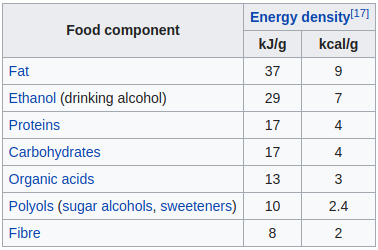
\includegraphics[width=0.5\textwidth]{calories.png}
\caption{\label{fig:cal} Summary of food energy.}
\end{figure}
\end{frame}

\begin{frame}{More practice with the force of friction, and human energies}
\begin{figure}
\centering
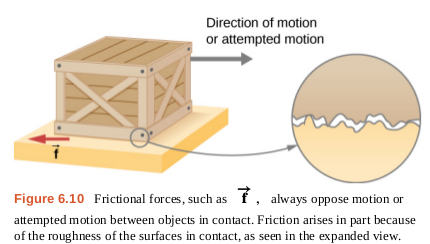
\includegraphics[width=0.7\textwidth]{friction.png}
\caption{\label{fig:f} Summary of friction.}
\end{figure}
\end{frame}

\begin{frame}{More practice with the force of friction, and human energies}
\begin{figure}
\centering
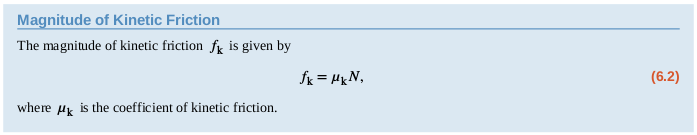
\includegraphics[width=0.9\textwidth]{friction2.png}
\caption{\label{fig:f2} Equation of friction.}
\end{figure}
\end{frame}

\begin{frame}{More practice with the force of friction, and human energies}
\begin{figure}
\centering
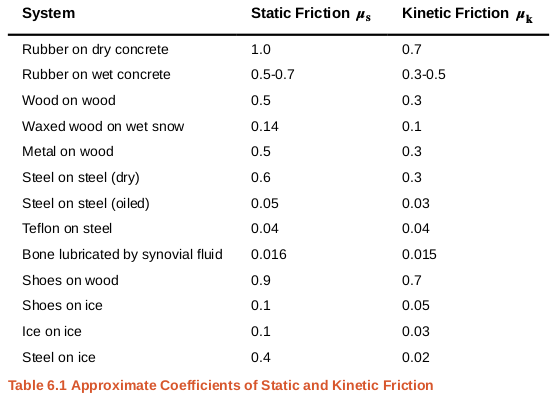
\includegraphics[width=0.9\textwidth]{friction3.png}
\caption{\label{fig:f2} Sumary of friction coefficients.}
\end{figure}
\end{frame}

\begin{frame}{More practice with the force of friction, and human energies}
\begin{figure}
\centering
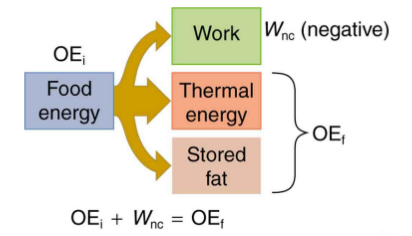
\includegraphics[width=0.6\textwidth]{human.png}
\caption{\label{fig:f3} Sumary of human power consumption.}
\end{figure}
\end{frame}

\begin{frame}{More practice with the force of friction, and human energies}
\begin{figure}
\centering
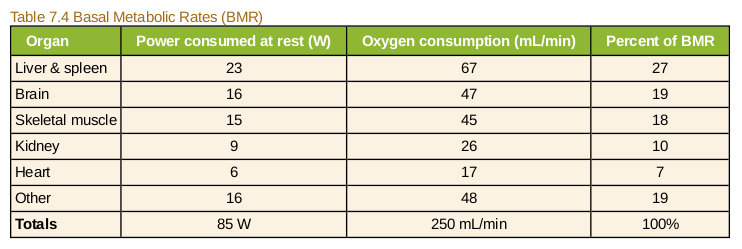
\includegraphics[width=0.8\textwidth]{human2.png}
\caption{\label{fig:f4} Sumary of human power consumption, part 2.}
\end{figure}
\end{frame}

\begin{frame}{More practice with the force of friction, and human energies}
\begin{figure}
\centering
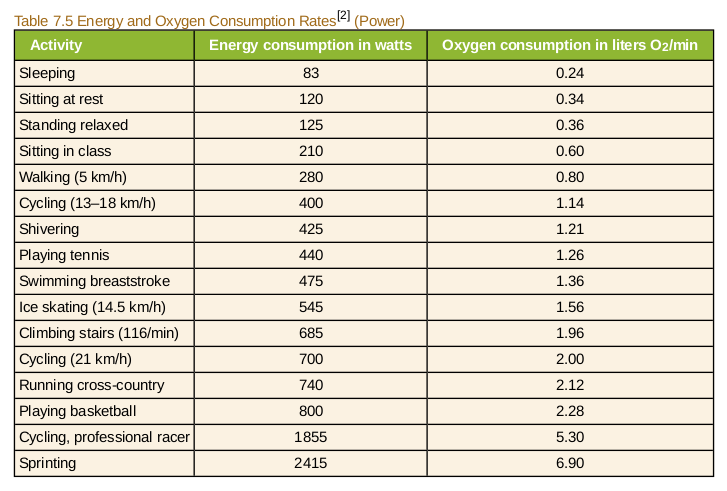
\includegraphics[width=0.8\textwidth]{human3.png}
\caption{\label{fig:f5} Sumary of human power consumption, part 3.}
\end{figure}
\end{frame}

\begin{frame}{More practice with the force of friction, and human energies}
\begin{figure}
\centering
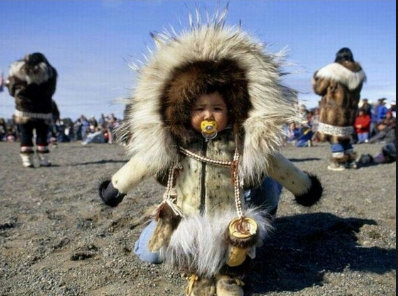
\includegraphics[width=0.8\textwidth]{inuit.png}
\caption{\label{fig:f6} Inuits: did you try ice, my friend?}
\end{figure}
\end{frame}

\end{document}
